\documentclass[]{tufte-handout}

% ams
\usepackage{amssymb,amsmath}

\usepackage{ifxetex,ifluatex}
\usepackage{fixltx2e} % provides \textsubscript
\ifnum 0\ifxetex 1\fi\ifluatex 1\fi=0 % if pdftex
  \usepackage[T1]{fontenc}
  \usepackage[utf8]{inputenc}
\else % if luatex or xelatex
  \makeatletter
  \@ifpackageloaded{fontspec}{}{\usepackage{fontspec}}
  \makeatother
  \defaultfontfeatures{Ligatures=TeX,Scale=MatchLowercase}
  \makeatletter
  \@ifpackageloaded{soul}{
     \renewcommand\allcapsspacing[1]{{\addfontfeature{LetterSpace=15}#1}}
     \renewcommand\smallcapsspacing[1]{{\addfontfeature{LetterSpace=10}#1}}
   }{}
  \makeatother

\fi

% graphix
\usepackage{graphicx}
\setkeys{Gin}{width=\linewidth,totalheight=\textheight,keepaspectratio}

% booktabs
\usepackage{booktabs}

% url
\usepackage{url}

% hyperref
\usepackage{hyperref}

% units.
\usepackage{units}


\setcounter{secnumdepth}{-1}

% citations

% pandoc syntax highlighting

% longtable

% multiplecol
\usepackage{multicol}

% strikeout
\usepackage[normalem]{ulem}

% morefloats
\usepackage{morefloats}


% tightlist macro required by pandoc >= 1.14
\providecommand{\tightlist}{%
  \setlength{\itemsep}{0pt}\setlength{\parskip}{0pt}}

% title / author / date
\date{}


\begin{document}





\includegraphics{https://assets.gitlab-static.net/uploads/-/system/project/avatar/2639401/bayes.jpg?width=64}

Inferência Bayesiana em R

Giuliano Netto Flores Cruz março, 2020

\hypertarget{introduuxe7uxe3o}{%
\section{Introdução}\label{introduuxe7uxe3o}}

Quando pensamos em aprender sobre o mundo a partir da coleta de dados,
estamos pensando em \emph{inferência}. A inferência é um tipo de
raciocínio por meio do qual saímos de simples amostras para
generalizações em termos de uma população (1). Alternativamente, podemos
entendê-la como uma ponte de via oposta àquela da probabilidade:
enquanto que a última liga um processo de geração de dados aos valores
observados, a primeira sai de dados observados para tentar estimar o
referido processo (Fig. 1).

\begin{figure}
\centering
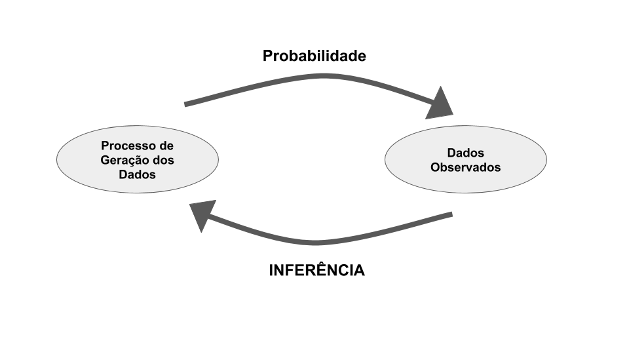
\includegraphics{imgs/fig1.png}
\caption{Fig. 1: Inferência é um tipo de raciocínio que liga amostras às
populações, isto é, dados observados aos processos responsáveis por
gerá-los. Adaptado de (2) - pág. IX.}
\end{figure}

Utilizando uma linguagem mais próxima à ciência da computação, chamamos
de inferência estatística ou \emph{aprendizado} o processo de usar dados
para inferir a distribuição que gerou estes mesmos dados (2) - daí,
também, termos populares em data science como \emph{learning},
\emph{statistical learning}, \emph{machine learning}, etc. Nesse
contexto, há duas grandes ``escolas'' que merecem destaque.

\begin{itemize}
\tightlist
\item
  \textbf{Inferência clássica}: também conhecida como
  \emph{frequentista}, é assim rotulada por sua predominância durante a
  primeira metade do século passado, impulsionada por seus tradicionais
  fundadores, como Karl Pearson e Ronald A. Fisher (3). Sob o paradigma
  clássico, é indispensável ter em mente que uma amostra \(x\) é apenas
  uma das muitas possíveis dentro de um conjunto amostral
  \(\mathcal{X}\). Tradicionalmente, entende-se que as observações
  \(X_1, X_2, \dots, X_n\) são \(n\) variáveis aleatórias, idependentes
  e igualmente distribuídas de acordo com uma distribuição
  \(\mathcal{D_0}\) descrita por p.d.f/p.m.f* \(f_0\).

  \begin{marginfigure}
  We know from \emph{the first fundamental theorem of calculus} that for
  \(x\) in \([a, b]\):
  \[\frac{d}{dx}\left( \int_{a}^{x} f(u)\,du\right)=f(x).\]
  \end{marginfigure}
\end{itemize}

Formula-se:

\[
X_1, X_2, \dots, X_n \overset{i.i.d.}{\thicksim} f_0
\]

\hypertarget{referuxeancias}{%
\section*{Referências}\label{referuxeancias}}
\addcontentsline{toc}{section}{Referências}

\hypertarget{refs}{}
\leavevmode\hypertarget{ref-Montgomery2016}{}%
1. Douglas C. Montgomery GCR. \emph{Estatistica aplicada e probabilidade
para engenheiros}. 6th ed. LTC (2016).

\leavevmode\hypertarget{ref-Wasserman2010}{}%
2. Wasserman L. \emph{All of statistics: A concise course in statistical
inference (springer texts in statistics)}. Springer New York (2004).

\leavevmode\hypertarget{ref-Paulino2018}{}%
3. Carlos Daniel Paulino BM M. Antonia Amaral Turkman. \emph{Estatística
bayesiana}. 2nd ed. Fundação Calouste Gulbenkian (2018).



\end{document}
